\section{Introducción}
El autocompletado por palabras estima qué término puede continuar un
contexto. Si una persona escribe ``el presidente del gobierno'', el
sistema calcula una distribución de posibles continuaciones. Una palabra
frecuente puede recibir probabilidad alta sin ser la continuación que esa
persona quería. Por ello se distinguen la distribución probabilística,
el orden de sugerencias y la utilidad real durante la escritura.

El objetivo de esta práctica es estudiar la recurrencia y el manejo de
memoria mediante una implementación verificable. Se compara una RNN
simple con una LSTM bajo el mismo corpus, vocabulario y presupuesto de
épocas. Un bigrama establece una referencia que solo utiliza la palabra
anterior. La pregunta experimental es si, con recursos modestos y un
contexto finito, la complejidad adicional de la LSTM produce una mejora
observable de pérdida y acierto léxico.

El interés industrial incluye sugerencias en editores y teclados,
asistencia a la redacción y puntuación de hipótesis de reconocimiento de
voz. Mikolov et al.~\cite{mikolov2010} estudian modelos recurrentes para
lenguaje y su aplicación al reconocimiento del habla. La presente
implementación no integra un teclado ni evalúa productividad de usuarios:
produce candidatos de la siguiente palabra y mide su calidad sobre texto
reservado. Tampoco completa una palabra parcialmente escrita. La entrada
``univers'' se trata como un token completo potencialmente desconocido.

Las contribuciones de este material son un procedimiento determinista de
preparación, código ejecutable, un protocolo registrado antes de consultar
prueba, resultados de diez entrenamientos y una demostración local.
Se evita equiparar una arquitectura con un resultado esperado: una LSTM
puede quedar por debajo de una RNN bajo ciertas decisiones de datos,
capacidad y optimización. La explicación debe partir de las observaciones
y reconocer qué hipótesis necesitarían nuevos experimentos.

\subsection{Estado de este documento}
Este texto es un \textbf{borrador asistido por inteligencia artificial}.
Los nombres identifican al grupo destinatario; no certifican que sus
integrantes hayan escrito, leído o validado el contenido. La guía exige
18--20 páginas técnicas, autoría propia y un máximo de 10\% de contenido
generado por IA. Este borrador no se presenta como cumplimiento de ese
límite ni como PDF final listo para el aula virtual. El grupo debe
investigar, redactar sus explicaciones, interpretar las pruebas y registrar
sus aportes. Parafrasear automáticamente este texto no acredita autoría.

\section{Marco teórico}
\subsection{Modelo probabilístico de lenguaje}
Para una secuencia de palabras $w_1,\ldots,w_T$, la regla de la cadena
permite escribir
\begin{equation}
 P(w_1,\ldots,w_T)=\prod_{t=1}^{T}P(w_t\mid w_{<t}).
\end{equation}
La práctica aproxima cada distribución condicional usando como máximo
$C$ tokens anteriores. Cada contexto se transforma en una matriz de
vectores aprendidos. El modelo neuronal devuelve $V$ puntuaciones o
\emph{logits}, que se convierten en probabilidades mediante
\begin{equation}
 p_j=\frac{\exp(z_j)}{\sum_{k=1}^{V}\exp(z_k)}.
\end{equation}
En el entrenamiento se usa entropía cruzada directamente sobre logits,
evitando implementar la exponencial y el logaritmo por separado.

Bengio et al.~\cite{bengio2003} proponen aprender representaciones
distribuidas y probabilidades de palabras conjuntamente. Su arquitectura
es de contexto fijo y no debe confundirse con una LSTM. En esta práctica,
la tabla de embeddings también se aprende desde cero. No se descargan
vectores preentrenados ni se aprovechan textos externos al corpus.

Un embedding asigna a cada identificador una fila de una matriz
$E\in\mathbb{R}^{V\times d}$. Dos palabras pueden adquirir vectores
parecidos cuando el entrenamiento encuentra que cumplen funciones
predictivas semejantes. Esto no equivale a una ontología explícita ni a
una garantía de comprensión semántica. La representación depende de los
ejemplos, la función objetivo y la frecuencia de cada palabra.

\subsection{Recurrencia y memoria de una RNN}
Una RNN simple actualiza un estado oculto a medida que lee tokens:
\begin{equation}
 h_t=\tanh(W_x x_t+W_h h_{t-1}+b).
\end{equation}
Los mismos parámetros se reutilizan en todas las posiciones. El estado
$h_t$ resume el prefijo observado; su dimensión permanece fija aunque
aumente la longitud del texto. La implementación usa una capa
unidireccional con activación tangente hiperbólica y estado inicial cero
para cada ventana. La red no accede a palabras futuras del objetivo.

La retropropagación a través del tiempo aplica la regla de la cadena a
las sucesivas actualizaciones. Un gradiente referido a una posición
lejana contiene productos de Jacobianos. Estos productos pueden reducir
o amplificar mucho la señal. Bengio et al.~\cite{bengio1994} analizan la
dificultad de aprender dependencias prolongadas mediante descenso por
gradiente. Esto expresa un problema de optimización, no la afirmación
de que todas las RNN fracasen en cualquier secuencia larga.

Pascanu et al.~\cite{pascanu2013} distinguen desvanecimiento y explosión
del gradiente. El recorte de norma reduce actualizaciones excesivas
cuando la norma supera un umbral; no reconstruye automáticamente una
señal ya desvanecida. En el código se aplica después de calcular
gradientes y antes de actualizar parámetros:
\begin{lstlisting}[language=Python]
loss.backward()
nn.utils.clip_grad_norm_(model.parameters(), 1.0)
optimizer.step()
\end{lstlisting}

\subsection{Celda y compuertas LSTM}
La LSTM distingue el estado de celda $c_t$ del estado oculto $h_t$.
La arquitectura original de Hochreiter y Schmidhuber~\cite{hochreiter1997}
introduce una vía para conservar información y facilitar el flujo del
error. Las variantes posteriores no son idénticas al diseño original.
Para interpretar la implementación moderna sin conexiones \emph{peephole},
se utilizan las siguientes ecuaciones:
\begin{align}
 i_t&=\sigma(W_i x_t+U_i h_{t-1}+b_i),\\
 f_t&=\sigma(W_f x_t+U_f h_{t-1}+b_f),\\
 g_t&=\tanh(W_g x_t+U_g h_{t-1}+b_g),\\
 o_t&=\sigma(W_o x_t+U_o h_{t-1}+b_o),\\
 c_t&=f_t\odot c_{t-1}+i_t\odot g_t,\\
 h_t&=o_t\odot\tanh(c_t).
\end{align}
La compuerta de olvido modula la retención del estado previo. La de
entrada regula la incorporación del candidato $g_t$, mientras que la de
salida controla qué parte de la celda se manifiesta en el estado oculto.
Las operaciones son por componente; una dimensión puede conservar
información mientras otra cambia. Las compuertas producen valores
continuos entre cero y uno y no decisiones simbólicas de verdadero o falso.

La actualización aditiva de la celda abre una trayectoria distinta a
la cadena de transformaciones no lineales de una RNN simple. Si una
compuerta de olvido permanece próxima a uno, puede conservarse información
a lo largo de varias posiciones. Esto no garantiza memoria infinita:
también importan los valores aprendidos, los datos y el horizonte de
entrenamiento. Sherstinsky~\cite{sherstinsky2020} desarrolla las ecuaciones
y fundamentos de ambas familias. La copia abierta consultada es una
revisión de 2023 del trabajo publicado en 2020.

Greff et al.~\cite{greff2017} comparan variantes de LSTM. Su formulación
incluye conexiones que no están presentes en la capa usada aquí. Por ello
se evita afirmar que la implementación reproduce exactamente ese estudio.
La referencia ayuda a distinguir decisiones arquitectónicas y a rechazar
la idea de una única configuración universalmente óptima.

\subsection{Memoria arquitectónica y ventana experimental}
La capacidad arquitectónica de conservar estado debe separarse del
contexto disponible en el experimento. Aunque una LSTM pueda procesar
secuencias largas, aquí recibe como máximo 4, 12 o 24 tokens y reinicia
sus estados entre ejemplos. Ninguna de las dos redes puede utilizar una
palabra que quedó fuera de esa ventana. Aumentar la memoria interna sin
ampliar el contexto no proporciona acceso al documento completo.

Sundermeyer et al.~\cite{sundermeyer2012} estudian LSTM para modelos de
lenguaje en tareas de inglés y francés. Sus resultados justifican la
pertinencia de la comparación, pero no permiten trasladar sus mejoras
numéricas a este corpus español. Doval et al.~\cite{doval2016} ofrecen
un antecedente en español que usa modelos de lenguaje para recuperar
segmentación de palabras. Su unidad de modelado es el carácter y su
objetivo es distinto al autocompletado de la siguiente palabra de esta
práctica.

\subsection{Regularización y comparación justa}
Se aplica dropout de probabilidad 0.15 al último estado válido antes de
la proyección al vocabulario. Durante entrenamiento se anulan
aleatoriamente componentes según ese mecanismo; durante evaluación se
desactiva. Srivastava et al.~\cite{srivastava2014} fundamentan dropout
como regularización. Aquí no se aplica una máscara recurrente dentro de
las compuertas, por lo que no se atribuyen al código propiedades de otras
variantes de dropout secuencial.

RNN y LSTM comparten dimensión de embedding, tamaño oculto, capa de salida,
datos y número de épocas. No comparten número exacto de parámetros ni
tiempo de cómputo. La LSTM posee más transformaciones por sus compuertas.
Por tanto, la comparación controla un conjunto concreto de decisiones,
pero no es una comparación a igual cantidad de parámetros ni a igual
presupuesto temporal. Esta distinción limita las conclusiones causales.

\subsection{Bibliotecas de Python empleadas}
\textbf{PyTorch 2.14.0+cpu} proporciona tensores, diferenciación automática,
capas neuronales, optimizadores y serialización. La clase
\texttt{nn.Embedding} transforma identificadores en vectores;
\texttt{nn.RNN} o \texttt{nn.LSTM} procesa el orden;
\texttt{nn.Linear} proyecta al vocabulario. El optimizador Adam realiza
las actualizaciones y \texttt{inference\_mode} evita construir el grafo
de gradientes durante inferencia. El método \texttt{eval()} desactiva
dropout: ambas operaciones cumplen funciones distintas.

\textbf{NumPy 2.5.3} organiza ventanas, selecciona índices de entrenamiento
y almacena matrices comprimidas. Se usa un generador con semilla para
elegir posiciones sin reemplazo. \textbf{Matplotlib 3.11.2} genera figuras
directamente desde los JSON de resultados. Las figuras no contienen
métricas simuladas ni valores reconstruidos visualmente.

La biblioteca estándar aporta \texttt{re} para tokenización,
\texttt{unicodedata} para normalización, \texttt{hashlib} para particiones
y huellas, \texttt{json} y \texttt{csv} para registros,
\texttt{pathlib} para rutas y \texttt{unittest} para pruebas.
\texttt{truststore} permite que el descargador use la confianza de
certificados del sistema. No se desactiva la verificación TLS.
\texttt{pypdf} sirve para comprobar materiales documentales y no participa
en entrenamiento. Quarto está disponible en el entorno, pero el informe
se compila con la clase oficial de LaTeX para conservar el formato exigido.

\section{Metodología y desarrollo práctico}
\subsection{Fuentes y trazabilidad}
Se seleccionaron doce publicaciones primarias con texto completo abierto.
La ficha de cada una registra enlace, pasajes pertinentes y uso previsto.
Las descargas conservan tamaño y SHA-256 en
\texttt{investigacion/acceso\_verificado.json}. Un hash permite comprobar
que se está revisando el mismo archivo, pero no acredita por sí solo su
calidad científica. La selección privilegia pertinencia y procedencia
académica, y conserva una fuente en español sin reemplazar trabajos
originales por resúmenes comerciales.

Las copias de autor de IEEE y Elsevier permiten leer gratuitamente los
trabajos manteniendo los datos de sus publicaciones. JMLR, PMLR, ISCA,
LREC y SEPLN complementan la selección. No se declara que las doce
publicaciones pertenezcan exclusivamente a IEEE, Springer o ScienceDirect.
La interpretación restrictiva de esa parte de la guía debe resolverla el
docente antes de cerrar la bibliografía. Las fichas documentan la revisión
de pasajes pertinentes y no afirman lectura integral por los integrantes.

\subsection{Corpus, licencia y unidad de análisis}
Se utiliza UD Spanish-AnCora, versión r2.17. AnCora contiene materiales
periodísticos y anotaciones lingüísticas~\cite{taule2008}; Universal
Dependencies ofrece un marco multilingüe de anotación~\cite{nivre2020}.
La práctica aprovecha el campo de texto y los identificadores de
documento y oración. No usa las etiquetas sintácticas como entradas ni
entrena un analizador de dependencias.

El archivo \texttt{LICENSE.txt} de la versión seleccionada establece
CC BY 4.0. Se conserva la atribución y se identifica la modificación:
normalización, deduplicación, nuevas particiones y selección de objetivos.
El README mantiene información histórica sobre licencias anteriores;
para esta distribución se sigue el archivo de licencia de r2.17.
Los artículos descargados para consulta no se redistribuyen
automáticamente con el código.

Se leen los tres archivos originales de corpus y se generan particiones
propias por documento. La unidad de predicción es una palabra superficial
normalizada. Leer \texttt{\# text} evita adoptar automáticamente la
segmentación de anotaciones que puede desdoblar contracciones. Así,
``del'' permanece una palabra. El procesamiento conserva palabras
funcionales: retirarlas destruiría continuaciones frecuentes necesarias
para la tarea.

\subsection{Normalización y vocabulario}
El procedimiento aplica minúsculas y Unicode NFC, conserva tildes,
transforma cantidades numéricas en \texttt{<num>} y omite puntuación.
No realiza stemming ni lematización. Estas decisiones reducen algunas
variantes y simplifican la salida, pero eliminan información de mayúsculas,
signos y números concretos. El sistema no puede recuperar fielmente
formato ni cantidades originales a partir de esa representación.

Los identificadores 0, 1 y 2 corresponden a PAD, UNK y BOS.
PAD rellena posiciones, UNK reúne términos fuera del vocabulario y BOS
marca el inicio de oración. Las restantes 2997 entradas se seleccionan
por frecuencia sobre todo el texto de entrenamiento; los empates se
resuelven alfabéticamente. Validación y prueba no incorporan palabras
nuevas a esa tabla. El vocabulario utiliza más texto de entrenamiento que
las 100000 posiciones seleccionadas para optimizar, algo explícito en
el diseño y compartido por los modelos.

La deduplicación global elimina 62 oraciones idénticas tras normalizar.
No detecta paráfrasis ni noticias similares. El orden de lectura es
determinista. La separación documental reduce fugas por oraciones del
mismo documento, aunque no garantiza independencia temática ni elimina
duplicación semántica entre noticias diferentes.

\subsection{Particiones y ejemplos causales}
Cada identificador documental se combina con el prefijo
\texttt{grupo5-v1:}. Se calcula SHA-256, se toman ocho dígitos
hexadecimales y se obtiene su residuo módulo 100. Valores menores que
80 asignan entrenamiento; de 80 a 89, validación; el resto, prueba.
El reparto es aproximado por documento, por lo que las proporciones
de palabras no tienen por qué ser exactamente 80/10/10.

\begin{table}[tb]
\caption{Corpus normalizado. Las particiones no son las del benchmark oficial.}
\label{tab:datos}
\centering
\setlength{\tabcolsep}{3pt}
\begin{tabular}{lrrr}
\toprule
 & Entrenamiento & Validación & Prueba\\
\midrule
Documentos & 1268 & 173 & 194\\
Oraciones & 13380 & 1971 & 2248\\
Palabras & 372317 & 52695 & 56796\\
Objetivos usados & 100000 & 52695 & 56796\\
OOV (\%) & 19.85 & 21.09 & 21.19\\
\bottomrule
\end{tabular}
\end{table}

Para cada posición se toma exclusivamente el prefijo de su oración.
Se antepone BOS y se conservan los últimos $C$ identificadores.
La palabra en esa posición es el objetivo. Por ejemplo, en ``el
presidente del gobierno'', el ejemplo con objetivo ``gobierno'' recibe
``BOS el presidente del''. Nunca se introduce ``gobierno'' en su propia
entrada ni se usa la oración siguiente. Los ejemplos del comienzo de
oración pueden tener menos de $C$ tokens.

Se rellenan a la derecha los contextos cortos con PAD y se conserva
su longitud real. La red procesa la matriz, pero se selecciona el estado
de la última posición real, no el estado correspondiente al último PAD.
Como la red es unidireccional, el relleno posterior no altera ese estado.
Una prueba automatizada comprueba esa invariancia en ambas arquitecturas.

La selección de 100000 objetivos de entrenamiento usa muestreo sin
reemplazo con semilla 20260929. Esto no son 100000 oraciones ni un nuevo
corpus independiente. Varias ventanas pueden proceder de una misma
oración y compartir prefijos. La evaluación usa todas las posiciones de
las particiones reservadas. Las semillas del modelo cambian inicialización
y orden de entrenamiento; no cambian el corpus ni su reparto.

\subsection{Arquitecturas implementadas}
La entrada tiene forma $B\times C$, donde $B$ es el tamaño de lote.
El embedding produce $B\times C\times48$ y la capa recurrente
$B\times C\times64$. Se extrae un vector de 64 componentes por
ejemplo, se aplica dropout durante entrenamiento y se proyecta a
3000 logits. PAD y BOS reciben una puntuación muy negativa porque
no representan palabras objetivo. UNK permanece en la distribución.

\begin{lstlisting}[language=Python]
values, _ = self.recurrent(self.embedding(x))
last = values[
    torch.arange(x.shape[0], device=x.device),
    lengths - 1
]
logits = self.output(self.dropout(last))
logits[:, PAD] = -1e9
logits[:, BOS] = -1e9
return logits
\end{lstlisting}

El embedding contiene $3000\cdot48=144000$ parámetros.
La salida contiene $3000\cdot64+3000=195000$.
La RNN agrega $64\cdot48+64\cdot64+2\cdot64=7296$
parámetros recurrentes. PyTorch mantiene dos vectores de sesgo.
El total es 346296. La LSTM multiplica por cuatro los términos
recurrentes y alcanza 368184 parámetros. La mayor parte de ambos
modelos reside en embedding y salida, no en las compuertas.

La diferencia absoluta es 21888 parámetros, alrededor de 6.32\%
respecto a la RNN. Esta proporción pequeña en el total no implica
igual costo por posición: la LSTM realiza varias transformaciones y
operaciones adicionales. Tampoco una cuenta de parámetros equivale
al tamaño exacto del archivo, que contiene metadatos y serialización.

\subsection{Referencia bigrama}
El bigrama cuenta transiciones de los mismos objetivos de entrenamiento
que reciben las redes. Para la palabra anterior $u$, se define
\begin{equation}
 P(w\mid u)=\frac{n(u,w)+\alpha q(w)}{n(u)+\alpha},
\end{equation}
donde $q$ es una distribución unigrama con pseudoconteo 0.1,
excluyendo PAD y BOS. Para un contexto sin observaciones, el resultado
es exactamente $q$. La suma de probabilidades es uno. Se elige
$\alpha\in\{1,10,100\}$ con la menor NLL de validación;
el valor seleccionado es 100. No se cambia al ver prueba.

Esta referencia no está diseñada para favorecer artificialmente a las
redes. Utiliza el mismo vocabulario y objetivos, aunque su capacidad
de generalizar contextos es distinta. La matriz de conteos densa tiene
$3000^2$ entradas: ser un modelo estadístico sencillo no significa
que su implementación concreta use poca memoria.

\subsection{Entrenamiento y selección}
El estudio principal ejecuta RNN y LSTM con $C=12$ y semillas 17,
29 y 43. La sensibilidad añade $C=4$ y $C=24$ para cada arquitectura
con semilla 17, diez entrenamientos en total. Un piloto de 2048
ejemplos y una época verifica funcionamiento y queda fuera de resultados.

Todos los entrenamientos finales usan cinco épocas, lotes de 512,
Adam con tasa 0.003 y recorte de norma 1. Se guarda el estado de la
época con menor NLL de validación. No hay parada temprana: se
ejecutan las cinco épocas y se selecciona el mejor punto guardado.
Se fijan semillas de Python, NumPy y PyTorch, dos hilos de CPU y
algoritmos deterministas cuando PyTorch los admite. Esto facilita
reproducción en el mismo entorno, pero no promete identidad binaria
en cualquier sistema operativo o versión de biblioteca.

La función de entrenamiento registra NLL, perplejidad y aciertos de
validación por época. Los archivos de resumen conservan configuración,
cantidad de parámetros, tiempo y versiones. El código se niega a
sobrescribir un modelo existente con el mismo identificador; para
repetir el estudio debe usarse una copia limpia o preservar los
resultados anteriores con una estructura explícita.

La carga usa \texttt{weights\_only=True}. Los primeros checkpoints
guardaron la versión de PyTorch como su tipo \texttt{TorchVersion};
se añadió compatibilidad explícita con ese tipo y una prueba de
carga completa. Las nuevas configuraciones guardan la versión como
cadena ordinaria. No se cambió ningún peso ni se repitió entrenamiento
para corregir ese problema de serialización.

\subsection{Métricas y tratamiento de desconocidas}
La pérdida media negativa logarítmica se expresa en nats:
\begin{equation}
 \mathrm{NLL}=-\frac{1}{N}\sum_{i=1}^{N}\log p(y_i\mid x_i),
 \qquad \mathrm{PPL}=\exp(\mathrm{NLL}).
\end{equation}
Una perplejidad menor indica mayor probabilidad geométrica de los
objetivos bajo esta codificación. Se calcula después de sustituir
palabras desconocidas por UNK. En consecuencia, no debe compararse
directamente con perplejidades de vocabularios, tokenizadores o corpus
distintos. Acertar UNK reduce pérdida, pero no identifica la palabra
original que deseaba escribir una persona.

El acierto top-$k$ léxico exige que el objetivo sea conocido y esté
entre los $k$ índices más probables:
\begin{equation}
 A_k=\frac{1}{N}\sum_{i=1}^{N}
 \mathbf{1}[y_i\ne\mathrm{UNK}\ \land\ y_i\in\mathrm{Top}_k(p_i)].
\end{equation}
Todas las posiciones permanecen en el denominador, incluidas las
desconocidas. La lista evaluada todavía puede contener UNK, que ocupa
un lugar sin generar un acierto léxico. La demo, en cambio, oculta
símbolos y muestra cinco palabras. Por tanto, el top-5 reportado
no es exactamente el acierto de las cinco sugerencias visibles:
es una métrica conservadora de la distribución original.

Con 21.19\% de objetivos desconocidos, el techo de acierto léxico
es aproximadamente 78.81\% aunque se acertaran todos los conocidos.
No se calcula F1 como si esta tarea fuese clasificación binaria de
sentimientos: la evaluación responde al objetivo de predecir una
palabra entre un vocabulario amplio. La utilidad con personas requeriría
medir aceptación de sugerencias, ahorro de pulsaciones y errores.

\subsection{Pruebas y reproducibilidad}
Ocho pruebas verifican normalización, separación documental,
correspondencia entre prefijos y objetivos, invariancia ante PAD,
tratamiento de UNK, normalización del bigrama, recuperación de pesos
y carga de checkpoint con metadatos. La comprobación de prefijos
revisa cien posiciones distribuidas de validación contra las oraciones
originales. No convierte ese muestreo en una demostración de ausencia
de todos los posibles errores.

Las pruebas terminaron correctamente el 29 de septiembre de 2026.
También se ejecutó el entrenamiento y la evaluación real completa.
La protección del archivo de prueba evita sobreescribirlo mediante
una segunda evaluación accidental, pero no es un sistema que impida
que una persona modifique el código. La disciplina metodológica y la
conservación de versiones siguen siendo necesarias.

\section{Resultados y discusión técnica}
\subsection{Comparación principal}
La Tabla~\ref{tab:resultados} resume 56796 posiciones de prueba.
Las filas neuronales son medias de tres semillas con contexto 12.
La tabla se genera directamente desde los JSON y conserva el mismo
denominador para todos los modelos.
\begin{table}[tb]
\caption{Resultados de prueba. RNN y LSTM: media de tres semillas.}
\label{tab:resultados}
\centering\begin{tabular}{lrrrr}
\toprule
Modelo & NLL & PPL & Top-1 (\%) & Top-5 (\%) \\
\midrule
Bigrama & 4.453 & 85.93 & 2.82 & 25.62 \\
RNN & 4.33 & 75.60 & 7.23 & 26.58 \\
LSTM & 4.36 & 78.15 & 6.72 & 26.14 \\
\bottomrule
\end{tabular}
\end{table}

La RNN alcanza perplejidad $75.60\pm0.36$ y la LSTM
$78.15\pm1.05$ (desviación estándar muestral). Frente al bigrama,
las reducciones relativas son aproximadamente 12.02\% y 9.05\%.
Sin embargo, el top-5 solo sube de 25.62\% a 26.58\% y 26.14\%.
Una mejora de probabilidad del objetivo puede ocurrir sin cambiar
mucho su posición entre los primeros candidatos. Las dos métricas
aportan información complementaria y no son porcentajes intercambiables.

El top-1 medio de la RNN es $7.23\pm0.56$\% y el de la LSTM,
$6.72\pm0.34$\%. Son valores bajos. La masa asignada a UNK y a
palabras funcionales limita la identificación del siguiente término.
No se oculta este resultado ni se renombra como ``precisión alta''.
El bigrama alcanza 2.82\% en esta definición de top-1 léxico.

\begin{figure*}[tb]
\centering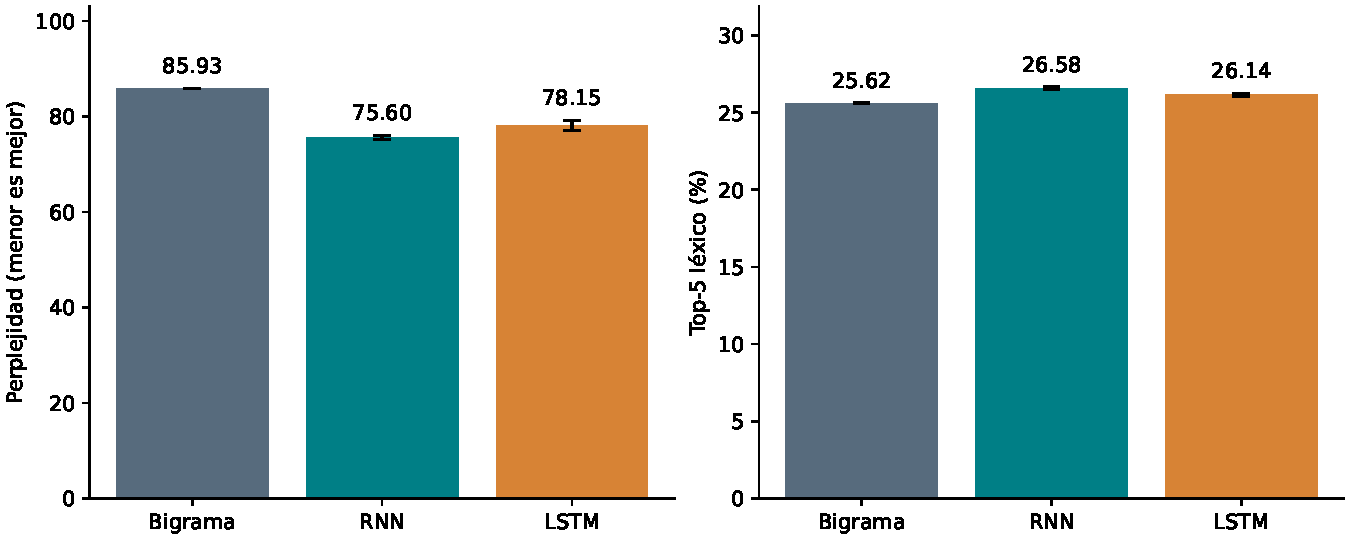
\includegraphics[width=.92\textwidth]{figuras/comparacion.pdf}
\caption{Comparación de prueba. Barras de error: desviación muestral entre
tres semillas para las redes; el bigrama tiene una configuración seleccionada.
La escala de perplejidad empieza en cero. Fuente: ejecución local registrada.}
\label{fig:comparacion}
\Description{Barras de perplejidad y acierto top-5. La RNN presenta menor perplejidad y mayor acierto que la LSTM bajo este protocolo.}
\end{figure*}

La RNN supera a la LSTM en las métricas medias de este protocolo.
No puede concluirse que la RNN sea intrínsecamente superior para todo
PLN. El entrenamiento es breve, los datos son limitados y la ventana
máxima es pequeña. Es plausible que esos factores reduzcan la utilidad
de memoria adicional, pero el experimento no aísla sus efectos.
Atribuir causalmente el resultado a uno requeriría nuevos controles.

Las tres semillas describen variación de optimización bajo una misma
partición; no son tres corpus independientes. No se realizaron pruebas
de significación ni intervalos de confianza sobre documentos. La
desviación entre semillas no cuantifica toda la incertidumbre de
generalización y no debe presentarse como margen de error poblacional.

\subsection{Aprendizaje y sensibilidad al contexto}
\begin{figure}[tb]
\centering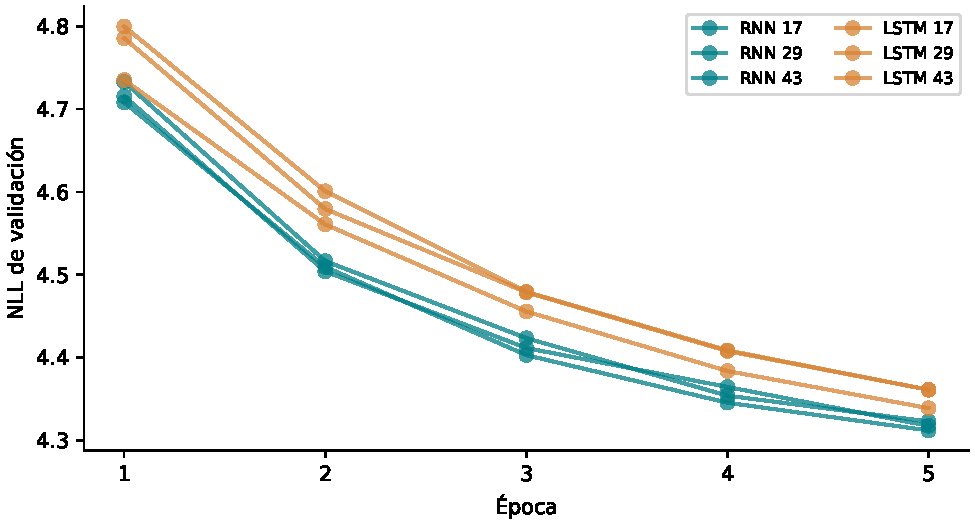
\includegraphics[width=\columnwidth]{figuras/aprendizaje.pdf}
\caption{NLL de validación por época, contexto 12. Cada línea corresponde
a una semilla. Los checkpoints se seleccionan por esta métrica.}
\label{fig:aprendizaje}
\Description{Seis curvas de pérdida de validación, correspondientes a tres semillas por arquitectura y cinco épocas.}
\end{figure}
La Figura~\ref{fig:aprendizaje} muestra las trayectorias de validación.
Es la evidencia apropiada para justificar la elección del checkpoint,
sin recurrir al resultado de prueba. Una disminución de pérdida en
cinco épocas no demuestra que el entrenamiento haya alcanzado su
óptimo. El presupuesto fijado permite comparar ejecuciones concretas,
no resolver una búsqueda exhaustiva de hiperparámetros.

\begin{table}[tb]
\caption{Sensibilidad exploratoria con semilla 17.}
\centering
\begin{tabular}{lrrr}
\toprule
Modelo & Contexto & PPL & Top-5 (\%)\\
\midrule
RNN & 4 & 75.49 & 26.50\\
RNN & 12 & 75.21 & 26.57\\
RNN & 24 & 75.73 & 26.54\\
LSTM & 4 & 78.30 & 26.05\\
LSTM & 12 & 78.82 & 26.04\\
LSTM & 24 & 78.46 & 25.99\\
\bottomrule
\end{tabular}
\end{table}
No aparece una mejora monótona al ampliar la ventana de 4 a 24.
El análisis contiene una sola semilla por contexto adicional, por lo
que se considera exploratorio. Tampoco compara textos sintéticos con
dependencias controladas a distancias conocidas. La ausencia de
mejora aquí no prueba que la LSTM carezca de memoria ni que las
dependencias distantes no importen en español.

\subsection{Costo y rendimiento}
El tiempo medio registrado para cinco épocas con contexto 12 es
78.17 segundos para RNN y 107.44 segundos para LSTM. Corresponde
a CPU con dos hilos e incluye evaluación de validación por época.
Los tiempos dependen de carga del equipo, biblioteca y longitud
efectiva; no deben convertirse en garantía de servicio o benchmark
universal de hardware.

Se registró también latencia de inferencia por modelo con lote uno,
diez calentamientos y cien consultas. El CSV conserva mediana y
el JSON añade percentil 95. La medición excluye carga de checkpoint,
tokenización y escritura de salida. La demo interactiva recarga el
modelo en cada consulta y, por tanto, su tiempo percibido incluye
trabajo no contabilizado por ese microbenchmark. Una versión destinada
a servicio debería mantener el modelo cargado y medir la ruta completa.

\subsection{Demostración y análisis de errores}
La LSTM de la demo se selecciona por menor NLL de validación:
\texttt{lstm\_c12\_s29.pt}. Se utiliza LSTM para ilustrar el mecanismo
del tema aunque la RNN obtenga mejor promedio en la comparación.
La selección de ese checkpoint no convierte a la LSTM en ganadora
del estudio. Para una entrada vacía, BOS permite proponer palabras
de comienzo; la primera sugerencia registrada es ``el'' con 14.21\%.

Para ``el presidente del gobierno'', la primera sugerencia registrada
es ``de'' con 13.77\%, mientras que UNK concentra 10.61\%.
Estas probabilidades no afirman verdad factual ni corrección completa
de una frase. Si una persona acepta varias sugerencias consecutivas,
puede producirse repetición y deriva. El entrenamiento se evalúa con
prefijos reales, no con cadenas largas de decisiones propias acumuladas.

El archivo de ejemplos incluye ``la universidad de'', ``los estudiantes
de software'' y ``Riobamba ESPOCH Chimborazo''. Los términos fuera
de vocabulario se enumeran explícitamente en la demo. Son pruebas
ilustrativas seleccionadas para observar comportamientos; no sustituyen
la evaluación exhaustiva ni son una muestra aleatoria de usuarios.
El grupo debe discutir si las sugerencias son gramaticales, si tienen
sentido contextual y cuándo el sistema debería abstenerse.

Las sugerencias omiten PAD, BOS y UNK, pero conservan las probabilidades
originales. No se renormalizan a cien por ciento para que cinco opciones
parezcan exhaustivas. El token \texttt{<num>} puede mostrarse como
categoría numérica: el sistema no sabe qué cifra exacta corresponde.
Esta limitación nace de la normalización y no se resuelve cambiando
la presentación del resultado.

\subsection{Amenazas a la validez}
La validez interna depende de la construcción causal de ventanas,
la separación de documentos y la selección por validación. Las pruebas
cubren invariantes importantes, pero la deduplicación exacta no descarta
noticias similares entre particiones. El vocabulario cerrado agrupa
palabras distintas en UNK y altera la dificultad de la distribución.

La validez externa es limitada: se modela prensa, con una versión
concreta del corpus, normalización específica y pocos recursos.
No hay evidencia directa sobre mensajes de estudiantes, español
ecuatoriano cotidiano, textos técnicos actuales o accesibilidad en
teclados. La evaluación no incluye personas ni datos privados.
Las publicaciones históricas sirven de fundamento, no de evidencia
de rendimiento de productos comerciales actuales.

La validez de comparación también exige reconocer decisiones que
quedaron fijas: la misma tasa de aprendizaje puede no ser óptima
para ambas redes; cinco épocas no igualan convergencia; tres semillas
no agotan la variabilidad. Una extensión debería registrar de antemano
su nueva búsqueda, mantener prueba independiente y comparar costos
además de exactitud. No se propone ajustar esta versión mirando
repetidamente el conjunto de prueba ya utilizado.

\section{Conclusiones}
La implementación permite estudiar cómo una RNN acumula estado y
cómo una LSTM regula una celda mediante compuertas. Ambas producen
una distribución sobre palabras y admiten demostración local reproducible.
La capacidad conceptual de memoria debe distinguirse del contexto
finito que realmente recibe el código.

En el protocolo ejecutado, la RNN obtiene menor perplejidad y mayor
acierto léxico medio que la LSTM. Ambas mejoran la perplejidad del
bigrama, mientras que la ganancia top-5 es inferior a un punto
porcentual. La conclusión depende de los datos y presupuesto usados;
no demuestra una jerarquía general entre arquitecturas.

La tasa de desconocidas de 21.19\% y los bajos aciertos top-1 muestran
que este prototipo tiene cobertura y utilidad limitadas. Es apropiado
como experimento educativo, pero su utilización productiva necesitaría
otra evaluación. Mejorar cobertura, estudiar más semillas o comparar
presupuestos de cómputo son trabajos futuros, no resultados realizados.

La reproducibilidad comprende corpus versionado, semillas, configuración,
archivos de resultados y pruebas de integridad. El dominio del grupo
debe evidenciarse mediante lectura, ejecución y explicación propias.
El material asistido no reemplaza ese trabajo ni certifica el límite
de contenido IA de la asignatura.

\section{Enlaces a recursos}
Publicación del repositorio y presentación: pendiente de autorización
de visibilidad y de verificación de las URL. No se incluyen enlaces
inventados. El código y los materiales están disponibles localmente.
Corpus: \url{https://github.com/UniversalDependencies/UD_Spanish-AnCora/tree/r2.17}.

Los textos completos gratuitos y los pasajes utilizados se detallan
en \path{investigacion/FUENTES_ABIERTAS.md}. Las referencias siguientes
incluyen sus enlaces académicos. Los identificadores DOI describen la
publicación; cuando la página editorial requiere pago, debe utilizarse
la copia abierta enlazada en las fichas.
